% !TEX encoding = UTF-8 Unicode

%
% Exemple de rapport
% par Pierre Tremblay, Universite Laval
% modifié par Christian Gagne, Universite Laval
% modifié par Francis Valois, Université Laval
% 31/01/2011 - version 1.4
%

%
% Modele d'organisation d'un projet LaTeX 
% rapport/      dossier racine et fichier principal
% rapport/fig   fichiers des figures
% rapport/tex   autres fichiers .tex
%

% ** Preambule **
%
% Ajouter les options au besoin :
%    - "ULlof" pour inclure la liste des figures, requis si "\begin{figure}" utilise
%    - "ULlot" pour inclure la liste des tableaux, requis si "\begin{table}" utilise
%
\documentclass[12pt,ULlof,ULlot]{ULrapport}

% Chargement des packages supplementaires (si absent de la classe)
\usepackage[utf8]{inputenc}
\usepackage[T1]{fontenc}
\usepackage[autolanguage]{numprint}
\usepackage{icomma}
\usepackage{subfigure}
\usepackage{graphicx}
\usepackage[absolute]{textpos}
\usepackage[final]{pdfpages}
\usepackage{listings} % For source code
\usepackage{color}
\usepackage{pdflscape}
\usepackage{multirow}
\usepackage{array}

% settings pour le listing de code
\lstset{
	tabsize=4,
	language=matlab,
        basicstyle=\scriptsize,
        %upquote=true,
        aboveskip={1.5\baselineskip},
        columns=fixed,
        showstringspaces=false,
        extendedchars=true,
        breaklines=true,
        prebreak = \raisebox{0ex}[0ex][0ex]{\ensuremath{\hookleftarrow}},
	frame=single,
        showtabs=false,
        showspaces=false,
        showstringspaces=false,
        identifierstyle=\ttfamily,
        keywordstyle=\color[rgb]{0,0,1},
        commentstyle=\color[rgb]{0.133,0.545,0.133},
        stringstyle=\color[rgb]{0.627,0.126,0.941},
	language=Java
}
\newcommand{\HRule}{\rule{\linewidth}{0.2mm}}
%\usepackage[hmargin=3cm,vmargin=3.5cm]{geometry}
\definecolor{mygrey}{gray}{.96} % Light Grey
\lstset{ 
	language=vhdl,              % choose the language of the code
%("language=Verilog" is popular as well)
	tabsize=4,			% sets the size of the tabs in spaces (1
%Tab is replaced with 3 spaces)
	basicstyle=\scriptsize,               % the size of the fonts that are
%used for the code
	numbers=left,                   % where to put the line-numbers
	numberstyle=\tiny,              % the size of the fonts that are used
%for the line-numbers
	stepnumber=1,                   % the step between two line-numbers. If
%it's 1 each line will be numbered
	numbersep=5pt,                  % how far the line-numbers are from the
%code
	backgroundcolor=\color{mygrey}, % choose the background color. You must add \usepackage{color}
	showspaces=false,              % show spaces adding particular underscores
	showstringspaces=false,        % underline spaces within strings
	%showtabs=false,                % show tabs within strings adding particular underscores
	frame=single,	                 % adds a frame around the code
	tabsize=3,	                    % sets default tabsize to 2 spaces
	captionpos=b,                   % sets the caption-position to bottom
	breaklines=true,                % sets automatic line breaking
	breakatwhitespace=false,        % sets if automatic breaks should only happen at whitespace
	%escapeinside={\%*}{*)},        % if you want to add a comment within your code
	%commentstyle=\color{RedBrick}   % sets the comment style
}

\def\dbar{{\mathchar'26\mkern-12mu d}} 
%\usepackage[options]{nom_du_package}

% Definition d'une commande pour presenter des cellules multilignes dans un tableau
\newcommand{\cellulemultiligne}[1]{\begin{tabular}{@{}c@{}}#1\end{tabular}}


% Definition de colonnes en mode paragraphe avec alignement ajustable
% Cette definition requiert le chargement du package "array"
%    - alignement horizontal, parametre #1 : - \raggedright (aligne a gauche)
%                                            - \centering (centre)
%                                            - \raggedleft (aligne a droite)
%    - alignement vertical, parametre #2 : - p (aligne en haut)
%                                          - m (centre)
%                                          - b (aligne en bas)
%    - largeur, parametre #3 : longueur
\newcolumntype{Z}[3]{>{#1\hspace{0pt}\arraybackslash}#2{#3}}

% Definitions des parametres de la page titre
\TitreProjet{Livrable 3 - Robot Kinocto}                         % Titre du projet
\TitreRapport{Design III}       % Titre du rapport
\Destinataire{M. Dominique Grenier, M. Luc Lamontagne et M. Abdelhakim Bendada}         % Nom(s) du destinataire
\TableauMembres{%                                     % Tableau des membres de l'equipe
   910\,058\,073  & Émile Arsenault \\\hline 
   908\,190\,985  & Philippe Bourdages \\\hline
   910\,098\,468  & Pierre-Luc Buhler \\\hline    
   998\,107\,355  & Diane Fournier \\\hline
   908\,318\,388  & Olivier Sylvain \\\hline
   910\,055\,897  & Daniel Thibodeau \\\hline
   910\,097\,879  & Francis Valois \\\hline
}
\DateRemise{4 avril 2013}                           % Date de remis


% Corps du document

\begin{document}

%   Chapitres

%!TEX root = ../rapport.tex
%!TEX encoding = UTF-8 Unicode

% Chapitres "Introduction"

% modifié par Francis Valois, Université Laval
% 31/01/2011 - version 1.0 - Création du document
\chapter{Diagrammes de classes}
	\label{s:classes}
	\addtolength{\evensidemargin}{-1in}	

\begin{figure}[htbp]
\centering
\label{fig:DiagrammeClasse}
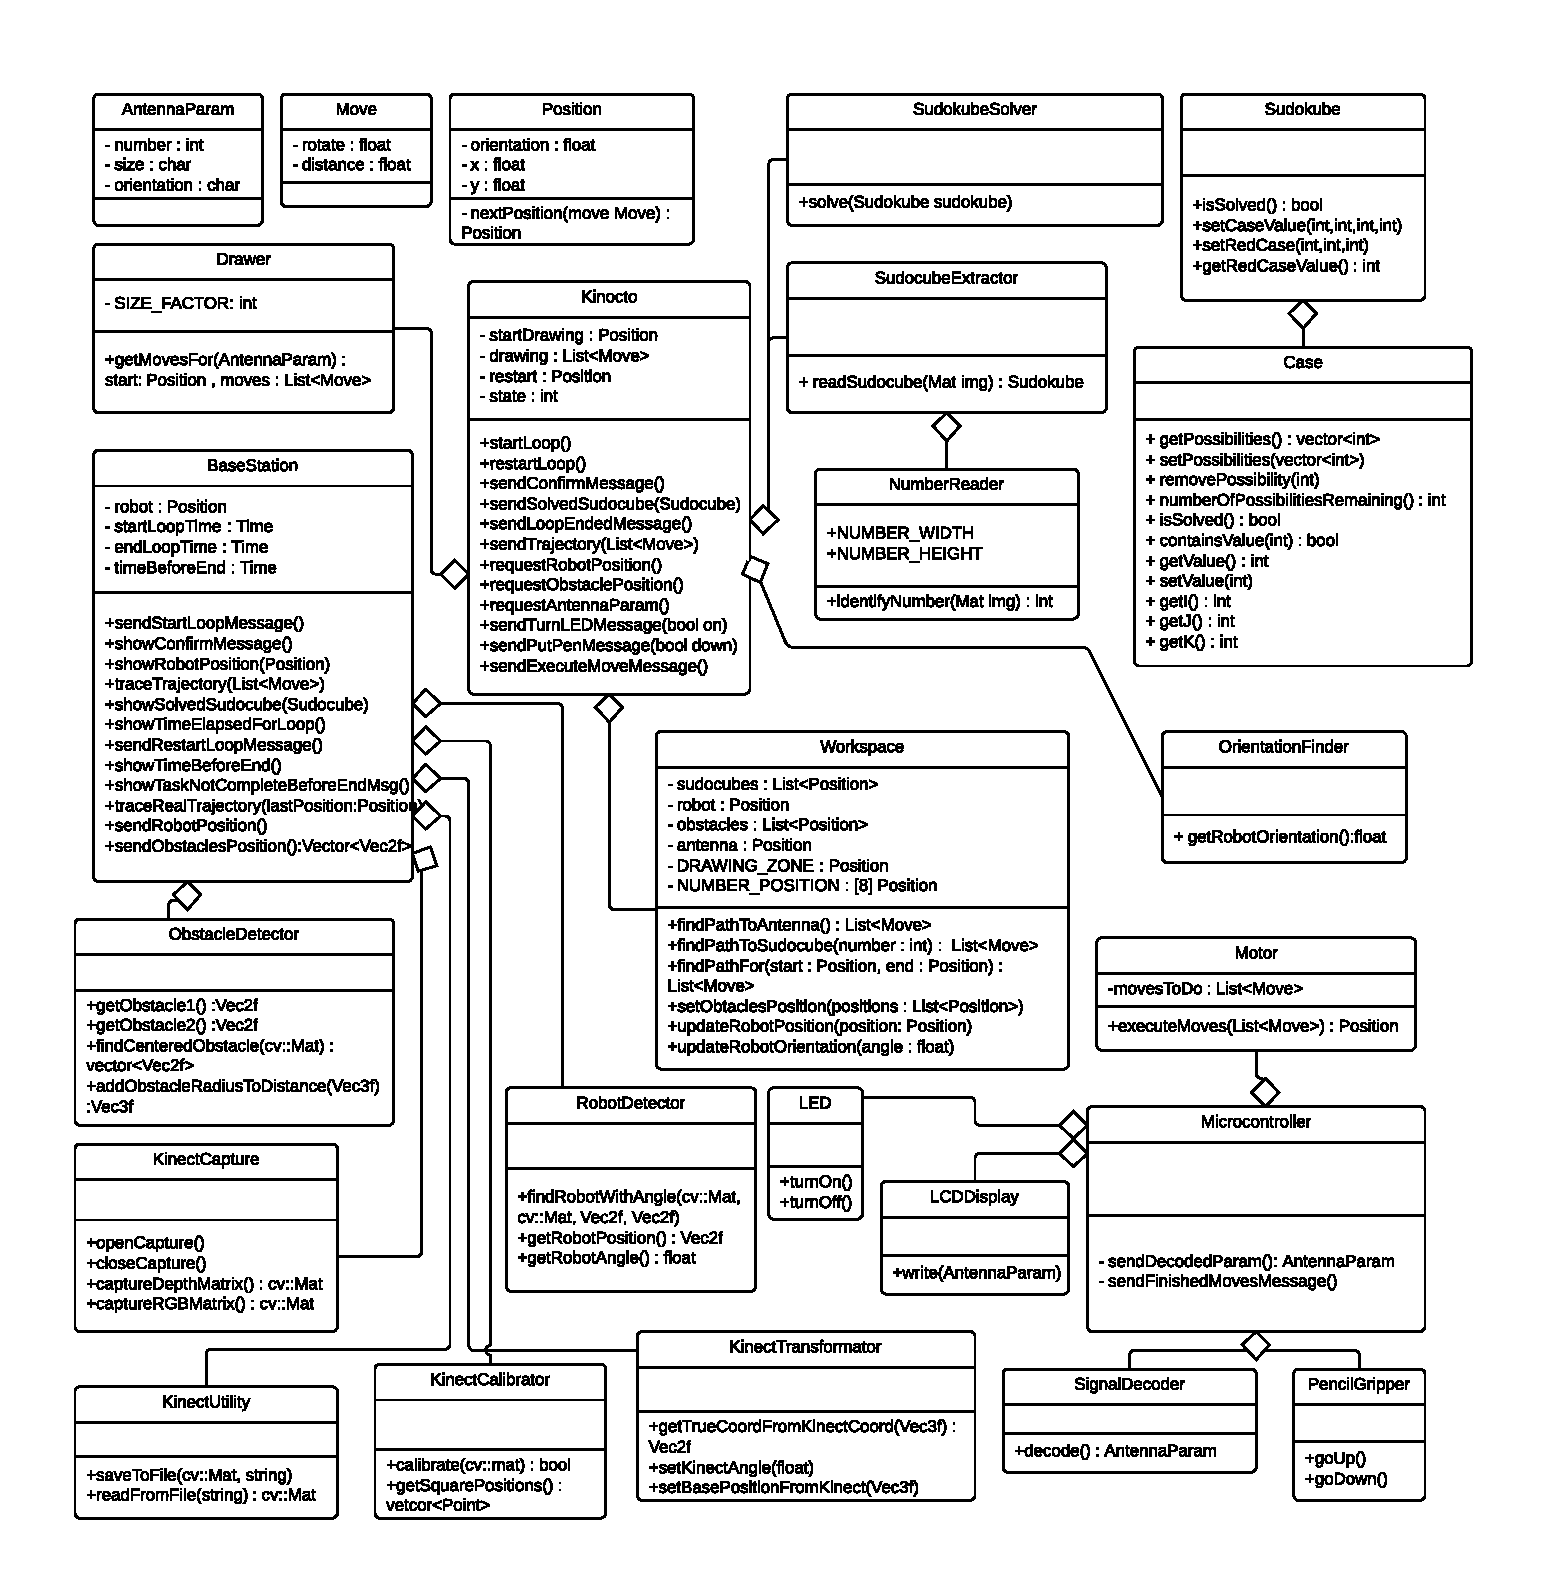
\includegraphics[scale=0.60]{fig/class_diagram.pdf}
\caption{Figure présentant le diagramme de classes du projet}
\end{figure}

%!TEX root = ../rapport.tex
%!TEX encoding = UTF-8 Unicode

% Chapitres "Introduction"

% modifié par Francis Valois, Université Laval
% 31/01/2011 - version 1.0 - Création du document

\chapter{Diagrammes de séquences}
\label{s:sequences}

%!TEX root = ../rapport.tex
%!TEX encoding = UTF-8 Unicode

% Chapitres "Introduction"

% modifié par Francis Valois, Université Laval
% 31/01/2011 - version 1.0 - Création du document

\chapter{Plan d'intégration}
\label{s:integration}
%!TEX root = ../rapport.tex
%!TEX encoding = UTF-8 Unicode

% Chapitres "Introduction"

% modifié par Francis Valois, Université Laval
% 31/01/2011 - version 1.0 - Création du document
\chapter{Registre de risques}
\begin{landscape}
\begin{table}[htbp]
	\small
 	 \centering
  	\caption{Registre de risques partie 1}
  	\scalebox{0.8}{
	\tabcolsep=0.11cm
    \begin{tabular}{|Z{\centering}{m}{1.5cm}||Z{\raggedright}{p}{3cm}|Z{\raggedright}{m}{1.5cm}|Z{\raggedright}{p}{5cm}|Z{\raggedright}{p}{4cm}|Z{\centering}{m}{1.5cm}|Z{\centering}{m}{1.5cm}|Z{\raggedright}{p}{4cm}|Z{\raggedright}{p}{3cm}|}\hline
    \textbf{Risque} &\textbf{Type de risque} &\textbf{Niveau de priorité (1- faible, 5-élevé)} & \textbf{Conséquences de l'occurrence du risque} & \textbf{Coût en performance associé au risque} & \textbf{Prob. d'occurrence (\%)} & \textbf{Coût estimé du risque (\$)}& \textbf{Plan de réduction du risque} & \textbf{Responsable du risque} \\\hline\hline
    1 & Bris  de la batterie Li-Po suite à une mauvaise utilisation & 5 & Plus d'autonomie énergétique pour le robot, opération impossible & L'ensemble du système sera inopérable &5 & 60 & Formation des utilisateurs à l'endroit de l'utilisation. Apposition d'un capteur de tension. Dispositifs de protection (fusibles) & É. Arsenault \\\hline
    2 & Bris  d'un ou des système d'alimentation & 5 & Les systèmes auxiliaires, le Mac mini ou les moteurs ne seront pas alimentés. Le système ne sera pas fonctionnel & Une partie ou l'ensemble du système sera inopérable & 5 & 25 & Utilisateur de connecteurs protégés (d'un seul sens possible). Dispositifs de protection (fusibles), surdimensionnement des composantes d'alimentation. Achat de pièces de rechange. & D. Thibodeau \\\hline
    3 & Bris  du crayon lors du dessin & 4 & Le dessin ne pourra être complété & La portion dessin sera partiellement complète & 20 & 2 & Tests rigoureux et optimisation du choix de crayon avant la compétition & É. Arsenault \\\hline
    4 & Bris du système de préhension & 5 & Le dessin ne pourra être complété et selon le moment du bris, la trajectoire du robot peut être affectée & La portion dessin sera partiellement complète et la trajectoire sera déviée & 5 & 10 & Tests rigoureux et essais multiples pour vérifier la stabilité en température lors du fonctionnement  & É. Arsenault \\\hline
    5 & Problèmes de réception ou de décodage du signal d'antenne & 4 & Si la réception est erronée, le robot peut exécuter sa séquence, mais l'exécution ne sera pas conforme au message. Si la réception est impossible, le système ne s'amorcera pas. & Accomplissement de la mauvaise tâche ou système non fonctionnel & 5 & 15 & Tests répétés pour un taux de succès de 100\% lors de la réception et du décodage avec ajout de sources de bruit externes. & D.Fournier \\\hline
   
    \end{tabular}}%
  \label{tab:rr1}%
\end{table}%
\end{landscape}
\begin{landscape}
\begin{table}[htbp]
	\small
 	 \centering
  	\caption{Registre de risques partie 2}
  	\scalebox{0.8}{
	\tabcolsep=0.11cm
    \begin{tabular}{|c||p{3cm}|>{\centering\arraybackslash}m{1.5cm}|p{4.8cm}|p{4.6cm}|>{\centering\arraybackslash}m{1.5cm}|>{\centering\arraybackslash}m{1.5cm}|p{4cm}|p{3cm}|}\hline
    \textbf{Risque} &\textbf{Type de risque} &\textbf{Niveau de priorité (1- faible, 5-élevé)} & \textbf{Conséquences de l'occurrence du risque} & \textbf{Coût en performance associé au risque} & \textbf{Prob. d'occurrence (\%)} & \textbf{Coût estimé du risque (\$)}& \textbf{Plan de réduction du risque} & \textbf{Responsable du risque} \\\hline\hline
    
    6 & Bris du pont en H & 5 & Les moteurs ne pourront être commandés correctement & Le robot ne peut pas se déplacer, le système n'est pas fonctionnel & 5 & 130 & Utilisation d'un régulateur de type PID afin d'éviter les appels brusques de courants, positionnement du pont de manière à limiter son exposition aux accrochages & F. Valois \\\hline
    
    7 & Bris d'une portion ou de la totalité du microcontrôleur & 4 & Le bris d'une portion du microcontrôleur empêche l'exécution de la tâche dans son ensemble et peut occasionner des bris dans les systèmes reliés & Un robot qui ne peut pas se déplacer correctement, qui n'allume pas la DEL ou qui n'active pas le préhenseur & 5 & 100 & Isolation des entrées et sorties avec des dispositifs de protection (diode), limiteur de courant & D. Fournier \\\hline
    
    8 & Bris du Mac mini & 5 & L'ensemble des auxiliaires ne fonctionnera pas correctement. Le système sera non fonctionnel & Robot incapable de se déplacer selon la trajectoire prévue et d'effectuer la tâche & 5 &  600  & Apposition de protections électriques (fusibles et interrupteurs) sur l'étage d'alimentation du Mac mini. Fixation robuste du Mac mini sur le robot. Protection du port USB du Mac mini en n'utilisant pas le fil d'alimentation. & F. Valois \\\hline
    
    9 & Caméra web désaxée & 3 & Les prises de données du sudo cube seront affectées & L'acquisition des données du sudo cube pourrait être non fonctionnelle et causer une erreur dans la résolution du cube & 10 &       & Tests rigoureux d'asservissement de la caméra et de retour à l'axe désiré suivant une modification externe. & P. Buhler \\\hline
    
    10 & Bris de la caméra web & 4 & Le bris de la caméra empêche la vision des cubes & Si la caméra ne peut voir le sudo cube, on ne peut trouver le chiffre dans la case rouge et effectuer le bon dessin & 5 & 80 & Storage adéquat de la caméra, protection d'alimentation (fusible), limiter les chocs contre les obstacles & D. Thibodeau \\\hline


    
\end{tabular}}%
  \label{tab:rr2}%
\end{table}%
\end{landscape}
\begin{landscape}
\begin{table}[htbp]
	\small
 	 \centering
  	\caption{Registre de risques partie 3}
  	\scalebox{0.8}{
	\tabcolsep=0.11cm
    \begin{tabular}{|c||p{3cm}|>{\centering\arraybackslash}m{1.5cm}|p{4cm}|p{4cm}|>{\centering\arraybackslash}m{1.5cm}|>{\centering\arraybackslash}m{1.5cm}|p{5cm}|p{3cm}|}\hline
    \textbf{Risque} &\textbf{Type de risque} &\textbf{Niveau de priorité (1- faible, 5-élevé)} & \textbf{Conséquences de l'occurrence du risque} & \textbf{Coût en performance associé au risque} & \textbf{Prob. d'occurrence (\%)} & \textbf{Coût estimé du risque (\$)}& \textbf{Plan de réduction du risque} & \textbf{Responsable du risque} \\\hline\hline

 	11 & Problème de communication entre le Mac mini et la station de base & 5 & Les informations requises ne pourront être transmises correctement, on perd l'information sur le comportement du robot ainsi que sa position. Le robot ne pourra pas se localiser initialement et en temps réel. & Le robot de remplira pas les exigences d'affichage sur la station de base, le robot ne recevra aucune position de la Kinect  & 5 &       & Tests répétés pour un taux de succès de près de 100\% lors de la transmission et de la réception de l'information en temps réel entre le Mac mini et la station de base & P. Bourdages \\\hline
 	12 & Bris du système d'exploitation du Mac mini & 4 & La portion logicielle du robot et le traitement seront absents. Le système ne sera pas fonctionnel & Robot incapable d'accomplir un traitement de tâches & 30 &       &Clonage d'une version fonctionnelle et stable du système d'exploitation & P. Buhler \\\hline
 	13 & Problème de communication entre le Mac mini et le microcontrôleur & 5 & L'ensemble des auxiliaires ne fonctionnera pas correctement. Le système sera non fonctionnel & Robot incapable de se déplacer selon la trajectoire prévue et d'effectuer la tâche & 5 &       & Tests répétés pour un taux de succès de près de 100\% lors de la transmission et de la réception de l'information entre le Mac mini et le microcontrôleur & D. Fournier \\\hline
 	14 & Contact avec un ou des obstacles & 3 & Bris du système et déviation de trajectoire possible & Un robot qui entre en contact avec les obstacles ne remplit pas les exigences du projet & 20 &       & Tests rigoureux sur les déplacements et marge de sécurité importante pour le contournement. & O. Sylvain \\\hline
    
    \end{tabular}}%
  \label{tab:rr3}%
\end{table}%
\end{landscape}

\begin{landscape}
\begin{table}[htbp]
	\small
 	 \centering
  	\caption{Registre de risques partie 4}
  	\scalebox{0.8}{
	\tabcolsep=0.11cm
    \begin{tabular}{|c||p{3cm}|>{\centering\arraybackslash}m{1.5cm}|p{4cm}|p{5cm}|>{\centering\arraybackslash}m{1.5cm}|>{\centering\arraybackslash}m{1.5cm}|p{4cm}|p{3cm}|}\hline
    \textbf{Risque} &\textbf{Type de risque} &\textbf{Niveau de priorité (1- faible, 5-élevé)} & \textbf{Conséquences de l'occurrence du risque} & \textbf{Coût en performance associé au risque} & \textbf{Prob. d'occurrence (\%)} & \textbf{Coût estimé du risque (\$)}& \textbf{Plan de réduction du risque} & \textbf{Responsable du risque} \\\hline\hline
	15 & Problème d'identification du robot et de l'environnement (vision) par la Kinect & 5 & Correction de la trajectoire erronée, risque de rencontrer les obstacles, mauvaise trajectoire calculée & La trajectoire réelle ne sera pas optimale et le robot risque de rencontrer des obstacles & 10 &  & Tests rigoureux et taux de succès de l'identification proche de 100\% & I. Mouhtij \\\hline
 	16 & Perturbations de l'environnement du robot (irrégularités sur la table ou dans l'éclairage) &2 & La trajectoire du robot pourrait être 			déviée si la vision est entachée par une mauvaise luminosité ou une irrégularité dans la table & La trajectoire parcourue par le robot ne 			sera pas idéale& 10 &  & Tests rigoureux des algorithmes de vision et d'asservissement, essais avec ajout d'irrégularités & D. Thibodeau 			\\\hline
 	    
    17 & Départ de l'un des membres de l'équipe & 3 & La quantité de tâches des membres restants de l'équipe devra être augmentée. & Des détails et des ajustements de pointes nécessitant plus de temps ne seront pas réalisés& 5 &       & S'assurer d'une bonne communication dans l'équipe et d'un bon transfert de conaissances& D. Thibodeau\\\hline
    
 
   \end{tabular}}%
  \label{tab:rr4}%
\end{table}%
\end{landscape}


%!TEX root = ../rapport.tex
%!TEX encoding = UTF-8 Unicode

% Chapitres "Introduction"

% modifié par Francis Valois, Université Laval
% 31/01/2011 - version 1.0 - Création du document

\chapter{Vision 1$^{ère}$ itération}
\label{vision1}

\section{Localisation avec la caméra embarquée}

La localisation avec la caméra embarquée est un système de localisation d'appoint dans le projet Kinocto. La classe Localisation doit recevoir une image et une orientation grossière selon le nord, sud, est ou ouest par rapport à la table. Elle doit ensuite être initialisée en fournissant un fichier .xml contenant les paramètres de calibration. Ces paramètres comprennent les paramètres intrinsèques de la caméra obtenus lors de la calibration, les paramètres liés à la distortion de l'image par la lentille, les paramètres extrinsèques qui permettent de lier les points des images prises par la caméra à leur position par rapport à un système de référence virtuel ainsi que les paramètres qui permettent de recadrer ces coordonnées par rapport au centre du robot.

Avec l'image et les paramètres provenant de la calibration, les méthodes de localisation, de détermination de l'orientation et de mesure de l'angle par rapport au mur peuvent être utilisées.

\subsection{Localisation}

\subsubsection{Transformations}

Pour effectuer la localisation du robot, il faut trouver dans l'image reçue au moins deux points identifiables dont les coordonnées par rapport à la table sont connues. Dans le projet Kinocto, ces points incluent les coins de la tables, les coins inférieurs des blocs de couleur, les coins du carré vert dessiné sur la table. Pour passer du système de coordonnée du robot à celui de la table, il faut résoudre le système d'équation suivant, où les points $P_1A$ et $P2_A$ sont les points dans le systèmes de la table, $P_1R$ et $P_2R$ sont les mêmes points dans le système du robot et $t_X$ et $t_Y$ sont les coordonnées du robot dans le système de la table:

\begin{equation}
\label{eq1}
X_{1A} = X_{1R}cos(\theta) - Y_{1R}sin(\theta) + t_X
\end{equation}
\begin{equation}
\label{eq2}
Y_{1A} = X_{1R}sin(\theta) + Y_{1R}cos(\theta) + t_Y
\end{equation}
\begin{equation}
\label{eq3}
X_{2A} = X_{2R}cos{\theta} - Y_{2R}sin(\theta) + t_X
\end{equation}
\begin{equation}
\label{eq4}
Y_{2A} = X_{2R}sin(\theta) + Y_{2R}cos(\theta) + t_Y
\end{equation}

En soustrayant l'équation~\ref{eq3} de l'équation~\ref{eq1} ainsi que l'équation~\ref{eq4} de l'équation~\ref{eq2}, on élimine $t_X$ et $t_Y$ et on se retrouve avec deux équations que l'on peut combiner pour obtenir une équation à une inconnue, $\theta$. Il s'agit d'une équation de la forme $a cos(\theta) + b sin(\theta) = c$. Ce type d'équation peut être résolu en considérant la relation suivante:

\begin{equation}
a cos(\theta) + b sin(\theta) = R cos(\theta - \alpha)
\end{equation}

Où $R = \sqrt{a^2 + b^2}$ et $tan(\alpha) = \frac{b}{a}$. En isolant $\theta$, on obtient donc:

\begin{equation}
\theta = cos^{-1}(\frac{c}{\sqrt{a^2 + b^2}}) + tan^{-1}(\frac{b}{a})
\end{equation} 

Il suffit ensuite d'utiliser $\theta$ dans deux des équation initiales pour retrouver les coordonnées du robot selon le système de référence de la table $t_X$ et $t_Y$.

\subsubsection{Localisation des points}

\begin{enumerate}
\item{Coins de table}

Les points correspondant aux coins de table sont trouvés dans l'image en effectuant d'abord une segmentation sur le noir et en utilisant ensuite l'algorithme des lignes de Hough pour retrouver les lignes de bas de mur. L'intersection entres les lignes de bas de mur constitue le coin de la table. Un intérêt de cette méthode est qu'elle permet de retrouver les coins de table même lorsqu'un obstacle se trouve devant celui-ci.

\item{Coins du bas des blocs de couleur}

Les coins du bas des blocs de couleurs peuvent être retrouvés en trouvant les intersections entre les lignes de bas de mur et la ligne du bas du bloc de couleur, trouvée après segmentation sur le bleu et l'orange.

\item{Coins du carré vert}

Les coins internes du carré vert peuvent être retrouvés en segmentant sur le vert et en retrouvant les intersections entre les lignes avec la méthode décrite plus haut.
\end{enumerate}

\subsection{Orientation et angle par rapport au mur}

L'angle par rapport au mur peut être utile pour réorienter le robot pour la lecture des sudokus. Il est facilement obtenu en utilisant la ligne de bas de mur détectée précédemment. L'orientation peut être déduite en utilisant cet angle et l'orientation fournie à l'initialisation.

\subsection{Extraire les contours d'un sudocube}

La première étape d'extraction consiste à segmenter par couleur verte afin d'isoler le cadre du sudocube. Puis, un algorithme de détection des contours est appliqué pour trouver deux polygones rectangulaires. Ces polygones sont les bordures intérieures et extérieures du cadre. L'aire des rectangles est calculée pour vérifier que les polygones sont assez grands pour être ceux du cadre.

Ensuite, à partir du polygone intérieur du cadre on isole une sous région de l'image principale. L'image obtenue est convertie en noir et blanc afin d'appliquer à nouveau un algorithme de contours afin de trouver les cases du sudocube. On sélectionne les polygones résultants selon leur aire. Si jamais le nombre de cases sélectionné n'est pas de 47 on recommence avec un seuil de tolérance différent pour l'algorithme de contour. Le polygone de la case rouge est obtenue en segmentant par couleur rouge et appliquant a nouveau un algorithme de contour. 

Finalement, les images des cases sont triées en fonction de leur position en X et en Y dans l'image du sudocube et un algorithme de reconnaissance des caractères appliqué sur toutes les cases afin d'identifier les numéros. L'algorithme de reconnaissance utilise la technique KNearest. Les chiffres trouvés sont ajoutés dans la structure de données du sudocube et la position de la case rouge est spécifiée.
%!TEX root = ../rapport.tex
%!TEX encoding = UTF-8 Unicode

% Chapitres "Introduction"

% modifié par Francis Valois, Université Laval
% 31/01/2011 - version 1.0 - Création du document

\chapter{Schémas électroniques 2$^{e}$ itération}
\label{electronics}
Le modèle de microcontrôleur employé est un Stellaris LM3S9B92. Les différentes entrées et sorties ont été fixées sur un circuit imprimé (PCB) dont le schéma est présenté à la figure \ref{fig:plan_micro}. 
\paragraph{}Tous les circuits électriques sont placés derrière un circuit de protection utilisant des fusibles dont le schéma est présenté à la figure \ref{fig:protection}. Ce circuit est prévu pour limiter les dégâts lors d'erreurs de manipulation ou de défectuosités électroniques. Par ailleurs, ces circuits sont actionnables par des interrupteurs placés devant les circuits respectifs. 
\paragraph{}L'alimentation 5V des périphériques est réalisée au moyen d'un circuit Buck 5V, le schéma est présenté à la figure \ref{fig:alim5V}.
\paragraph{}L'alimentation 24V du préhenseur et du Mac mini est réalisée au moyen d'un circuit Boost acheté chez un détaillant, pour lequel on ne dispose pas du plan de circuit en raison du secret d'ingénierie du fournisseur. La tension de sortie est variable avec un potentiomètre. La tension d'entrée est directement celle de la batterie. Une photo du dispositif est disponible à la figure \ref{fig:alim24Vphoto}.
\paragraph{}Le circuit de démodulation du signal Manchester émis sur les tables est réalisé au moyen du circuit présenté à la figure \ref{fig:manchester}. La clef de ce circuit est le LM567 qui est un circuit intégré permettant de syntoniser le signal d'antenne selon une largeur de bande que l'on établit au moyen des capacités présentes sur les différentes pines du LM567. Le LM567 permet d'isoler directement l'enveloppe du signal. Un comparateur à hystérésis est placé à la sortie du LM567 de manière à rendre plus uniformes et abruptes les transitions dans le signal d'enveloppe. 
\paragraph{}Le circuit de commande du préhenseur est présenté à la figure \ref{fig:prehenseur}. Il n'est composé que d'un transistor Mosfet qui permet d'activer la conduction du préhenseur (avec un courant proche de 150mA), directement à partir du microcontrôleur. Une diode de roue libre permet de décharger l'énergie de la bobine (préhenseur) lors des transitions.
\paragraph{}Le circuit de commande de la DEL est présenté à la figure \ref{fig:del_verte}. Il n'est composé que d'un transistor Mosfet qui permet d'activer la conduction de la DEL, une résistance de 100$\Omega$ permet de limiter le courant dans la DEL.

\begin{figure}
\centering
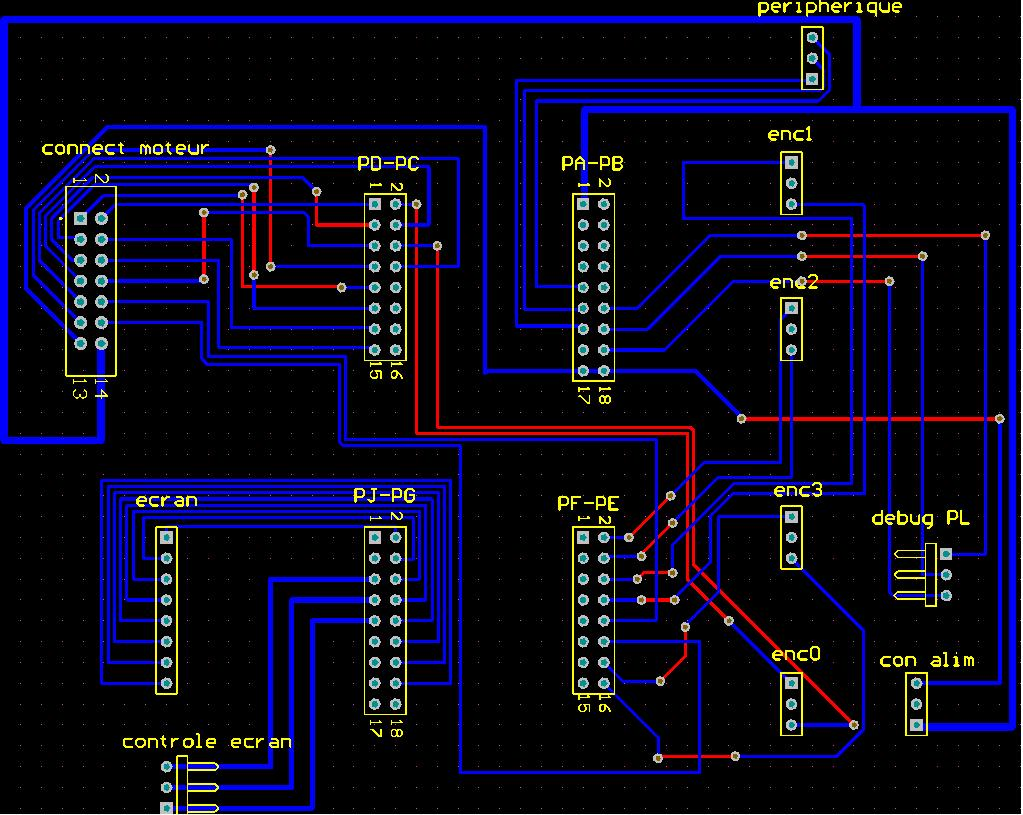
\includegraphics[scale=0.5]{fig/plan_micro.jpg}
\caption{Figure présentant le plan de l'alimentation 5V pour les périphériques}
\label{fig:plan_micro}
\end{figure}

\begin{figure}
\centering
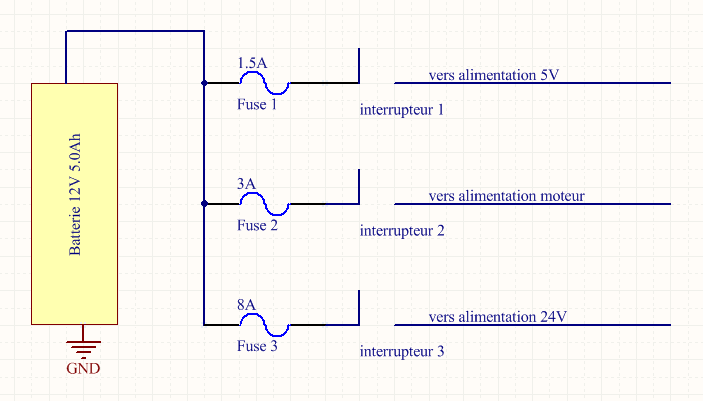
\includegraphics[scale=0.5]{fig/plan_circuit_protection.png}
\caption{Figure présentant le circuit de protection des circuits électriques}
\label{fig:protection}
\end{figure}

\begin{figure}[htbp]
\centering
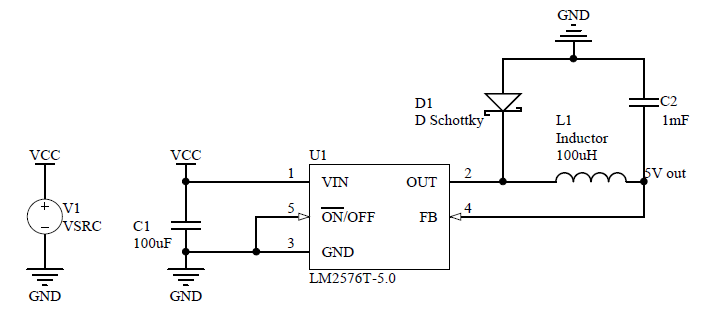
\includegraphics[scale=0.5]{fig/alim_5V.png}
\caption{Figure présentant le plan de l'alimentation 5V pour les périphériques}
\label{fig:alim5V}
\end{figure}

\begin{figure}[htbp]
\centering
\includegraphics[scale=0.1]{fig/alim_24V_photo.png}
\caption{Figure présentant une photo de l'alimentation 24V achetée telle quelle}
\label{fig:alim24Vphoto}
\end{figure}

\begin{figure}[htbp]
\centering
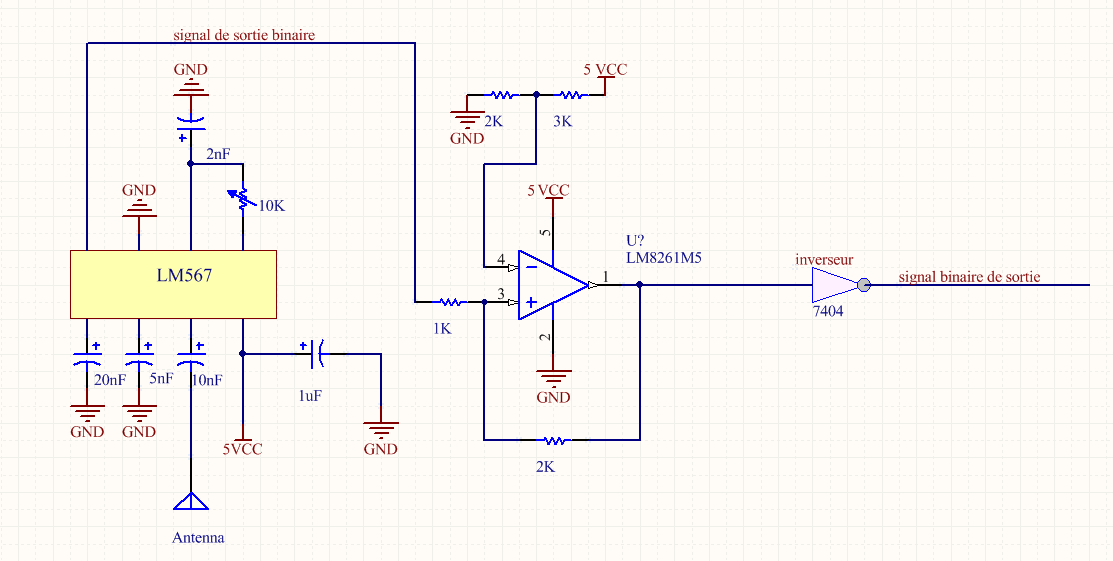
\includegraphics[scale=0.5]{fig/plan_manchester.png}
\caption{Figure présentant le plan du récepteur Manchester}
\label{fig:manchester}
\end{figure}

\begin{figure}[htbp]
\centering
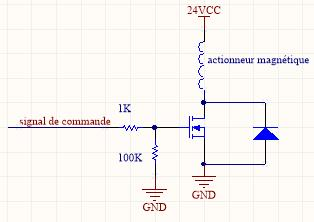
\includegraphics[scale=0.5]{fig/prehenseur.jpg}
\caption{Figure présentant le plan du circuit de commande du préhenseur}
\label{fig:prehenseur}
\end{figure}

\begin{figure}[htbp]
\centering
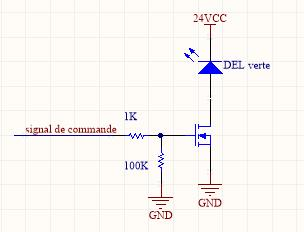
\includegraphics[scale=0.5]{fig/del_verte.jpg}
\caption{Figure présentant le plan du circuit de commande de la DEL verte}
\label{fig:del_verte}
\end{figure}

%\appendix
%%!TEX root = ../rapport.tex
%!TEX encoding = UTF-8 Unicode
% Chapitres "Annexes"

% modifié par Francis Valois, Université Laval
% 31/01/2011 - version 1.0 - Création du document
\chapter{Annexes}
\label{s:annexes}

\section{Asservissement des moteurs}
\subsection{Fonction agissant comme PID} \label{s:fonction_PID}
\begin{lstlisting}[language=C]
long PIDHandler(volatile long *consigne, volatile long *measured_value, volatile float *I, volatile long *previous_error, float dt)
{
  long error = *consigne - *measured_value;
  *I = *I + error*dt;
  float D = (error - *previous_error)/dt;
  long output = Kp*error + Ki*(*I) + Kd*D;
  *previous_error = error;
  return output;
}
\end{lstlisting}



\end{document}
% Fin du document

